\section{Hbase:}

HBase est un  des composants additionnels d’Apache. Pour les systèmes de gestion de base de données (SGBD) orientés colonne, soit en “No-SQL”, la notion de base de données et la façon dont les données sont stockées sont très différentes des systèmes de gestion de bases de données relationnelles.

Apache HBase est un data store orienté colonne utilisant des paires clé/valeur. La base de données HBase s’installe généralement sur le système de fichiers HDFS (pour Hadoop Distributed File System).

\begin{figure}[h]
	\centering
    
\includegraphics[scale=0.6]{img/part3/2.1}
    \caption{Logo Hbase}
\end{figure}

\subsection{Installation d'Hbase:}

Pour l'installation de Hbase , il est très important de vérifier si Java et Hadoop ont été bien installés sur le système.

\begin{enumerate}

\item On commence par télécharger Hbase a partir de son archive officiel( \url{https://hbase.apache.org/downloads.html})et On décompresse ce dernier (on a choisi la version 1.4.9).

\item On Crée deux dossiers dans le répertoire racine et les nommé "HBase" et "zookeeper".

\item Maintenant, nous devons modifier 2 fichiers, accédez à l'emplacement décompressé.

\textbf{- 1er fichier :} Modifiez \texttt{hbase-config.cmd} , situé dans le dossier bin sous l'emplacement décompressé et ajoutez la ligne ci-dessous pour définir :
\begin{figure}[h]
	\centering
    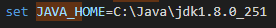
\includegraphics[scale=0.6]{img/part3/2.2}
    \caption{modifier le fichier hbase-config.cmd}
\end{figure}

\textbf{- 2eme fichier :} Modifiez \texttt{hbase-site.xml} , situé dans le dossier conf sous l'emplacement décompressé et ajoutez la section ci-dessous
\begin{figure}[h]
	\centering
    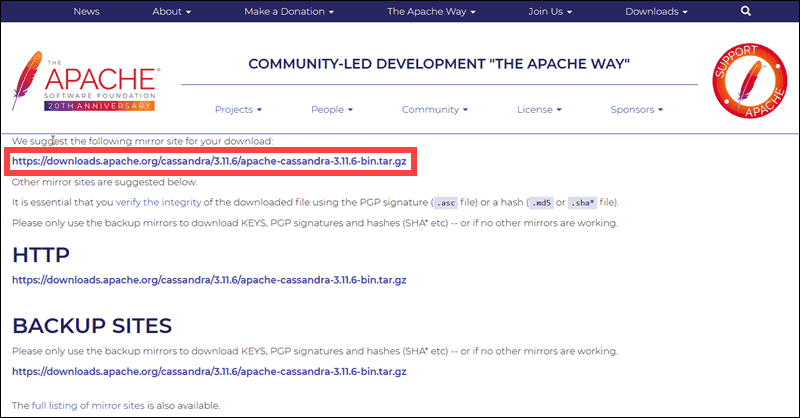
\includegraphics[scale=0.4]{img/part3/2.3}
    \caption{Modifier le fichier hbase-site.xml}
\end{figure}

\end{enumerate}









